\section{Introduction}

\begin{frame}
\frametitle{Why to model?}

\begin{block}{External use}
A model documents the interface: informs users on how the component would interact with other components.
\end{block}
\pause
\begin{block}{Internal use}
A model sets expectations: lets developers clarify the desired behavior of the component.
\end{block}
\end{frame}

\begin{frame}
\frametitle{The Unified Modeling Language}
It includes several diagrams in the following categories:
\begin{block}{Structure diagrams}
They are concerned with the parts that statically compose the system.
Examples: {\em class}, {\em component}
\end{block}
\pause
\begin{block}{Behavior diagrams}
They are concerned with what the system dynamically performs.
Examples: {\em activity}, {\em state}, {\em timing}, {\em sequence}
\end{block}
\end{frame}

\begin{frame}
\frametitle{Diagrams you are already familiar with}

\begin{block}{Class}
When you model a software application using the object-oriented paradigm.
\end{block}
\begin{block}{State}
When you describe the behavior of a circuit with a state machine.
\end{block}
\begin{block}{Activity}
When your behavior is based on logical decisions, especially if cycles are present.
\end{block}
\begin{block}{Timing}
When you write down the temporal evolution of (interdependent) signals.
\end{block}
\end{frame}

\begin{frame}
\frametitle{Diagrams of interest}

\begin{block}{To be discussed here:}
\begin{itemize}
\item Component
\item Sequence
\item State
\end{itemize}
\end{block}

\begin{block}{Reference tools:}
\begin{itemize}
\item Violet: \url{http://alexdp.free.fr/violetumleditor/page.php}
\\ for Component (using the Object diagram) and Sequence
\item Dia: \url{http://argouml.tigris.org}
\\ for Component and State (both using the UML sheet)
\end{itemize}
\end{block}

\end{frame}

\section{Diagrams}

\subsection{Component}

\begin{frame}
\frametitle{Component diagram}
\framesubtitle{At a glance}

Stereotype notation (on Violet):
\begin{figure}
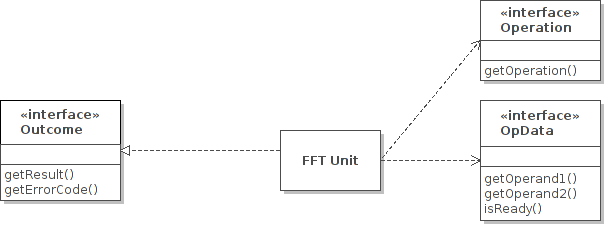
\includegraphics[width=0.6\textwidth]{lecture02/img/stereotype_components.png}
\end{figure}
Ball-and-socket notation (on Dia):
\begin{figure}
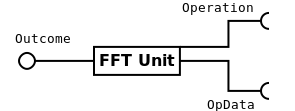
\includegraphics[width=0.4\textwidth]{lecture02/img/ballsocket_components.png}
\end{figure}


\end{frame}

\begin{frame}
\frametitle{Component diagram}
\framesubtitle{Isolated components}

\begin{figure}
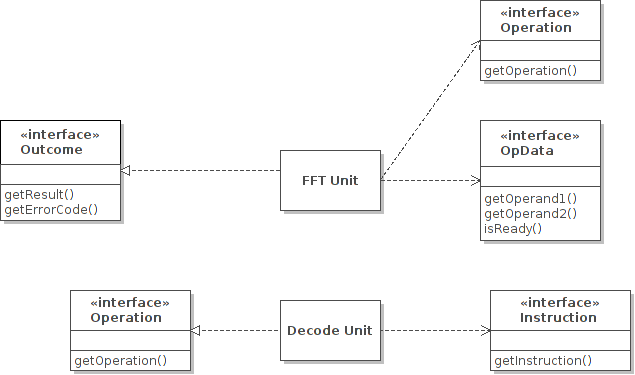
\includegraphics[width=0.7\textwidth]{lecture02/img/isolated_components.png}
\end{figure}

\begin{block}{Two components with their I/O interfaces}
We decouple the implementation from the way the component interacts with the rest of the system
\end{block}
\end{frame}

\begin{frame}
\frametitle{Component diagram}
\framesubtitle{Connected components}

\begin{figure}
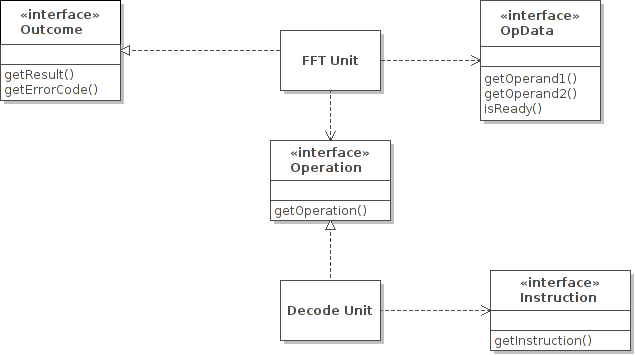
\includegraphics[width=0.6\textwidth]{lecture02/img/connected_components.png}
\end{figure}
\begin{figure}
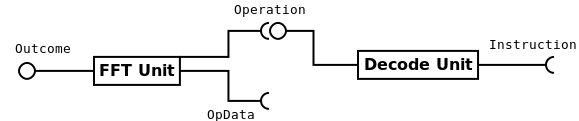
\includegraphics[width=0.5\textwidth]{lecture02/img/ballsocket_connected_components.png}
\end{figure}


\begin{block}{Component match their implemented/required interfaces}
It means we can substitute one component with another one having the same interface
\end{block}
\end{frame}

\begin{frame}
\frametitle{Component diagram}
\framesubtitle{Interfaces}

\begin{block}{Two categories of interfaces: {\em implemented} and {\em required}}
\begin{itemize}
\item implemented: other components will call its methods; a component that implements such interface is also called a {\em realization}
\item required: this component will call its methods; the interface for such component is also called a {\em dependency}
\end{itemize}
\end{block}
\pause
\begin{block}{Two kinds of methods: getters and setters}
\begin{itemize}
\item getter: the method is used to retrieve data
\item setter: the method is used to inject data
\end{itemize}
\end{block}

\end{frame}

\begin{frame}
\frametitle{Component diagram}
\framesubtitle{When to rely on setters rather than getters?}

\begin{block}{Setters allow to notify events to a component}
\begin{itemize}
\item The component that requires the interface will be the originator of the event
\item If no setters exist, all components must periodically check for input data: synchronous logic instead of asynchronous logic
\end{itemize}
\end{block}

\end{frame}

\begin{frame}
\frametitle{Component diagram}
\framesubtitle{Adding a bus}

\begin{figure}
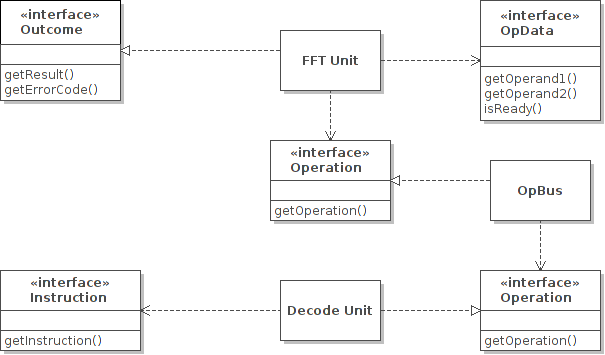
\includegraphics[width=0.7\textwidth]{lecture02/img/connected_components_bus.png}
\end{figure}

\begin{block}{The addition of a bus component does not break compatibility}
Note how interfaces may be both implemented and required
\end{block}
\end{frame}

\begin{frame}
\frametitle{Component diagram}
\framesubtitle{Summarizing}

\begin{block}{Component diagrams define the separation between parts of a system}
As soon as the interface is stabilized, the other components do not need to concern with the actual implementation.
\end{block}
\end{frame}

\subsection{Sequence}

\begin{frame}
\frametitle{Sequence diagram}
\framesubtitle{At a glance}

\begin{figure}
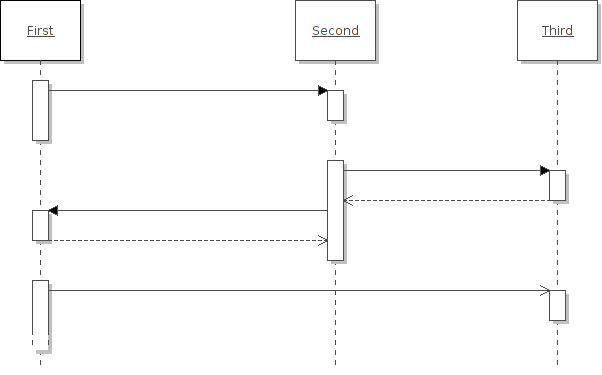
\includegraphics[width=0.7\textwidth]{lecture02/img/abstract_sequence.png}
\end{figure}

\begin{itemize}
\item There are multiple participants that exchange synchronous or asynchronous messages
\item The time axis is vertical, pointing down
\end{itemize}
\end{frame}


\begin{frame}
\frametitle{Sequence diagram}
\framesubtitle{Synchronous messages}

\begin{figure}
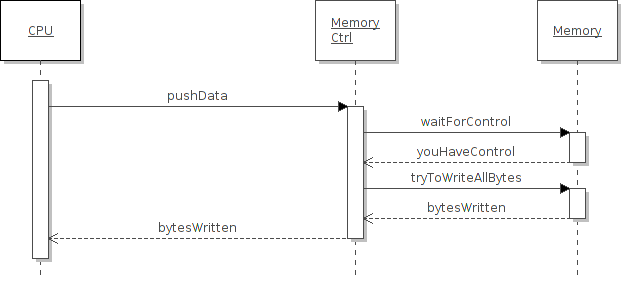
\includegraphics[width=0.7\textwidth]{lecture02/img/memory_sync.png}
\end{figure}

\begin{block}{Synchronous messages require to wait for return}
\begin{itemize}
\item They are represented with full arrows, with return arrows optional
\item The bar length refers to the duration of the operation
\end{itemize}
\end{block}
\end{frame}

\begin{frame}
\frametitle{Sequence diagram}
\framesubtitle{Asynchronous messages}

\begin{figure}
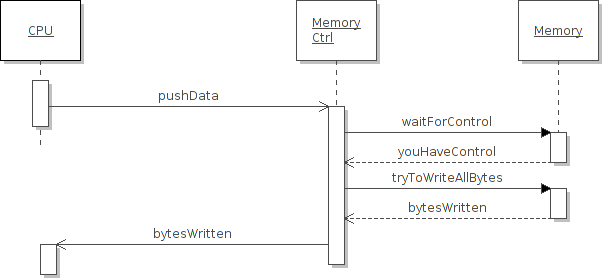
\includegraphics[width=0.7\textwidth]{lecture02/img/memory_async.png}
\end{figure}

\begin{block}{Asynchronous messages do not have returns}
\begin{enumerate}
\item The CPU issues the message and moves to other activities
\item As soon as the memory controller completes, it notifies the CPU by either creating an event or setting some flag
\item The CPU either interrupts its operation or, at some point, checks the flag
\end{enumerate}
\end{block}
\end{frame}

\begin{frame}
\frametitle{Sequence diagram}
\framesubtitle{Summarizing}

\begin{block}{Sequence diagrams deal with transactions}
\begin{itemize}
\item They focus on components and show how they dynamically interact using messages
\item Compared to timing diagrams, they better point out the duration of an operation and the consequent wait times
\end{itemize}
\end{block}
\end{frame}

\subsection{State}

\begin{frame}
\frametitle{State diagram}
\framesubtitle{At a glance}

\begin{figure}
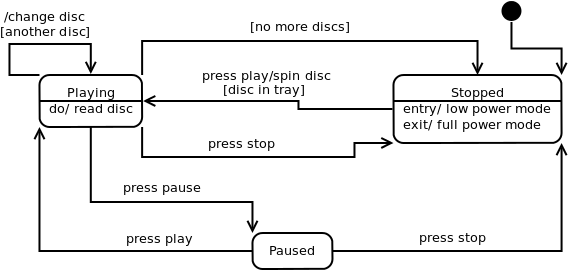
\includegraphics[width=0.7\textwidth]{lecture02/img/compactdisc_state.png}
\end{figure}

\only<1>{
\begin{block}{Annotations on transitions:}
\begin{itemize}
\item \texttt{label}: {\em event} that causes the transition
\item \texttt{[label]}: {\em guard}, i.e., condition that must be satisfied to perform the transition
\item \texttt{/label}: {\em action} to be performed during the transition
\end{itemize}
\end{block}
}
\only<2>{
\begin{block}{Annotations on states:}
\begin{itemize}
\item \texttt{entry/label}: action to be performed as we enter the state
\item \texttt{do/label}: action to be cyclically performed within the state
\item \texttt{exit/label}: action to be performed as we leave the state
\end{itemize}
\end{block}
}
\end{frame}

\begin{frame}
\frametitle{State diagram}
\framesubtitle{In the context of digital systems}

\begin{itemize}
\item Event: an input signal changes to a given value (or performs a given transition)
\item Guard: an internal signal (i.e., a state variable) changes to a given value
\item Transition action: we write a new value to an output signal
\item Entry action: we initialize some internal signals and/or load data
\item Exit action: we free/reset resources and/or save data
\end{itemize}
\end{frame}

\begin{frame}
\frametitle{State diagram}
\framesubtitle{Summarizing}

\begin{block}{State diagrams define the evolution of state information}
They capture information related to both events and actions
\end{block}
\end{frame}